\chapter{EDA Lab II: The MBA Placement Dataset, End to End}
\companion{InfoEdge DS interview experience: the Round 3 placement task (at 2:39)}{https://youtu.be/nWyBQhGnHaM?t=159}

This is the dataset reported in InfoEdge Round 3. We walk through the full EDA exactly as you would narrate it in the Colab round, with code, real
printed output and plots. Notebook section: \emph{Case 1} of \code{EDA\_Lab.ipynb}.
\begin{trap}[: about the numbers in this chapter]
The real file is Kaggle's ``Campus Recruitment'' \code{Placement\_Data\_Full\_Class.csv} (215 students). It could not be downloaded inside this build
environment, so the outputs below come from a \textbf{simulated replica with the same 15 columns and similar structure} (generated by
\code{eda\_lab/make\_placement\_replica.py}, seed 42). Put the real CSV next to the notebook and every cell runs unchanged; your numbers will differ
in detail, but the method, the checks and the leakage finding are the same.
\end{trap}

\section{The data dictionary}
\begin{center}\small
\begin{tabularx}{\linewidth}{l l X}
\toprule
Column & Type & Meaning\\
\midrule
\code{sl\_no} & ID & serial number (drop for modelling)\\
\code{gender} & nominal & M / F\\
\code{ssc\_p}, \code{ssc\_b} & numeric, nominal & 10th-grade percentage and board (Central / Others)\\
\code{hsc\_p}, \code{hsc\_b}, \code{hsc\_s} & numeric, nominal, nominal & 12th-grade percentage, board, stream (Commerce / Science / Arts)\\
\code{degree\_p}, \code{degree\_t} & numeric, nominal & undergraduate percentage and field (Comm\&Mgmt / Sci\&Tech / Others)\\
\code{workex} & binary & prior work experience\\
\code{etest\_p} & numeric & employability test percentage\\
\code{specialisation}, \code{mba\_p} & nominal, numeric & MBA specialisation (Mkt\&Fin / Mkt\&HR) and MBA percentage\\
\code{status} & \textbf{target} & Placed / Not Placed\\
\code{salary} & numeric & offered package, \emph{recorded only after placement}\\
\bottomrule
\end{tabularx}
\end{center}
\textbf{Frame}: one row is a student; the decision is made \emph{before} placement season (e.g. whom to coach), so only information available then may be used.

\section{Step 1: load and look}
\begin{lstlisting}
pl = pd.read_csv("Placement_Data_Full_Class.csv")      # or make_placement_replica()
print(pl.shape)
overview(pl)
\end{lstlisting}
\outlabel
\begin{lstlisting}[style=out]
(215, 15)
                  dtype  missing  missing_%  n_unique     example
sl_no             int64        0        0.0       215           1
gender              str        0        0.0         2           F
ssc_p           float64        0        0.0       207       52.67
ssc_b               str        0        0.0         2      Others
hsc_p           float64        0        0.0       212       56.04
hsc_b               str        0        0.0         2      Others
hsc_s               str        0        0.0         3     Science
degree_p        float64        0        0.0       203       57.82
degree_t            str        0        0.0         3    Sci&Tech
workex              str        0        0.0         2          No
etest_p         float64        0        0.0       185        98.0
specialisation      str        0        0.0         2      Mkt&HR
mba_p           float64        0        0.0       202        72.4
status              str        0        0.0         2  Not Placed
salary          float64       69       32.1       102    263000.0
\end{lstlisting}
\textbf{Say}: ``215 students, 15 columns, 5 numeric scores, 7 categoricals, an ID, the target, and salary. Only salary has missing values: 69 of them, 32\%. That
number is suspicious: it is close to the share of non-placed students, so I will check whether salary is missing \emph{because} the student was not placed.''

\section{Step 2: data quality}
\begin{lstlisting}
print("duplicate rows:", pl.duplicated().sum(), "| duplicate ids:", pl["sl_no"].duplicated().sum())
pct = ["ssc_p", "hsc_p", "degree_p", "etest_p", "mba_p"]
print("all percentages inside [0, 100]:", ((pl[pct] >= 0) & (pl[pct] <= 100)).all().all())
\end{lstlisting}
\outlabel
\begin{lstlisting}[style=out]
duplicate rows: 0 | duplicate ids: 0
all percentages inside [0, 100]: True
\end{lstlisting}
Every percentage lies in its valid range. Therefore a 96.9 in \code{hsc\_p} is a topper, not an error: \textbf{no outlier deletion} (the ``presence of mind'' test from the
reported interview).

\section{Step 3: the target}
\begin{lstlisting}
pl["status"].value_counts(), pl["status"].value_counts(normalize=True)
\end{lstlisting}
\outlabel
\begin{lstlisting}[style=out]
Placed 146 (0.679)    Not Placed 69 (0.321)
\end{lstlisting}
Mildly imbalanced (68/32). Accuracy is usable, but report precision, recall and F1 for the class the decision is about, and use stratified splits.

\section{Step 4: salary, leakage and ``if the package is given, we know the outcome''}
\subsection{The check}
\begin{lstlisting}
pl.groupby("status")["salary"].apply(lambda s: s.isna().mean())
rule = np.where(pl["salary"].notna(), "Placed", "Not Placed")
print("Accuracy of 'salary present => Placed':", (rule == pl["status"]).mean())
pd.crosstab(pl["salary"].notna().rename("salary_present"), pl["status"])
\end{lstlisting}
\outlabel
\begin{lstlisting}[style=out]
status
Not Placed    1.0
Placed        0.0
Name: fraction_salary_missing
Accuracy of 'salary present => Placed': 1.0
status          Not Placed  Placed
salary_present
False                   69       0
True                     0     146
\end{lstlisting}

\subsection{What it means, said properly}
\begin{itemize}
\item Salary is missing for \textbf{100\%} of non-placed students and \textbf{0\%} of placed ones. So the single rule ``if a package is recorded, the student was placed''
  is \textbf{100\% accurate}. Any model given \code{salary} (or even ``salary is missing'') will find this and score near-perfect AUC.
\item This is \textbf{target leakage}: salary is a \emph{consequence} of being placed, recorded after the outcome. When the model is used (before placements), no student has a
  salary yet, so the feature does not exist and the near-perfect offline score would collapse.
\item The missingness is not MCAR or MAR; it is structural (``not applicable''): there is no salary to impute for a non-placed student. Imputing it (with the median) would be
  meaningless and would still leak through the imputed pattern.
\item \textbf{Decision}: drop \code{salary} (and anything derived from it) from the placement model. This is the first thing the successful candidate said in Round 3.
\item Salary is still valuable for a \emph{different} question: ``what package will a placed student get?''. That is a regression on placed students only (or a two-part
  model: $P(\text{placed})\times\E[\text{salary}\mid\text{placed}]$, Chapter 4).
\end{itemize}

\subsection{Salary EDA among placed students}
\begin{lstlisting}
placed = pl[pl["status"] == "Placed"].copy(); s = placed["salary"]
print(s.describe().round(0))
print("skew:", round(s.skew(), 2), "| skew of log(salary):", round(np.log(s).skew(), 2))
q1, q3 = s.quantile([.25, .75]); upper = q3 + 1.5 * (q3 - q1)
print(f"IQR upper fence = {upper:,.0f}; packages above it: {(s > upper).sum()}")
placed.groupby("workex")["salary"].median(), placed.groupby("gender")["salary"].median()
\end{lstlisting}
\outlabel
\begin{lstlisting}[style=out]
count 146  mean 315623  std 98410  min 200000  25% 253000  50% 305000  75% 339000  max 784000
skew: 2.39 | skew of log(salary): 0.98
IQR upper fence = 468,000; packages above it: 6
workex  No 286500   Yes 311000          gender  F 275000   M 312000
\end{lstlisting}
\begin{center}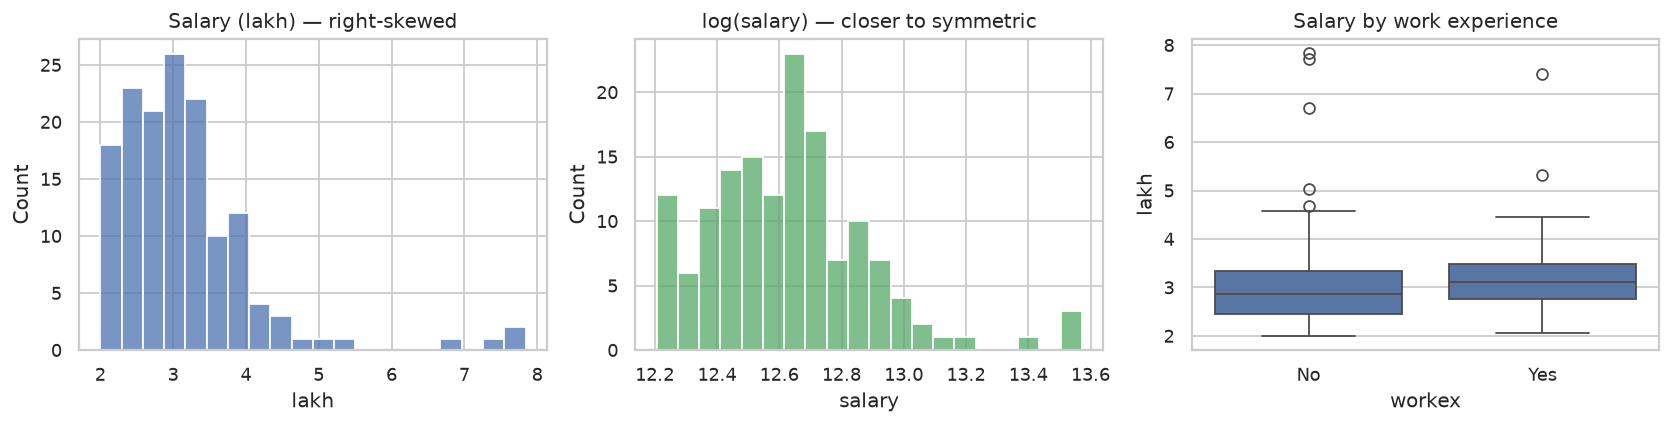
\includegraphics[width=\linewidth]{eda_lab/figs/pl_salary.png}\end{center}
\textbf{Reading}: salary is strongly right-skewed (mean 3.16 lakh $>$ median 3.05 lakh; skew 2.4) with a floor at 2 lakh and six packages above the IQR fence, the highest 7.84 lakh.
These are plausible genuine offers, so keep them; for a salary model use $\log(\text{salary})$ (skew drops to about 1) or a Gamma/quantile objective, and report MAPE.
Work experience is associated with higher packages. A gender gap in medians appears; with 146 rows and no controls it is a \emph{question to investigate} (does it persist
after controlling for specialisation and scores?), not a conclusion.

\section{Step 5: univariate analysis of the scores}
\begin{lstlisting}
num_summary(pl[pct])
\end{lstlisting}
\outlabel
\begin{lstlisting}[style=out]
          count   mean    std   min    25%    50%    75%    max  skew  kurt  n_iqr_outliers  n_zeros
ssc_p     215.0  66.92  10.79  40.0  59.58  67.57  73.73  89.40 -0.11 -0.32               0        0
hsc_p     215.0  66.21  11.24  37.0  57.91  67.43  73.88  96.87 -0.23 -0.07               0        0
degree_p  215.0  66.52   7.64  50.0  60.95  67.03  71.72  83.63 -0.07 -0.55               0        0
etest_p   215.0  72.97  12.38  50.0  63.74  73.18  80.80  98.00  0.08 -0.53               0        0
mba_p     215.0  62.28   5.42  51.2  58.31  62.15  66.11  76.00  0.07 -0.59               0        0
\end{lstlisting}
\begin{center}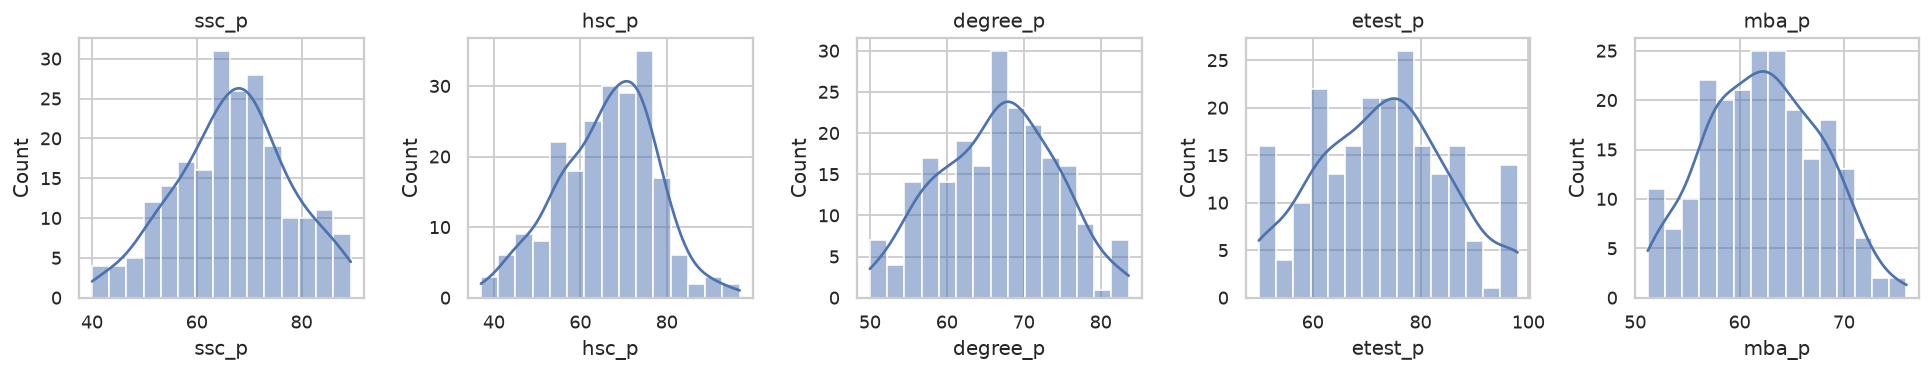
\includegraphics[width=\linewidth]{eda_lab/figs/pl_hist.png}\end{center}
\textbf{Reading}: all five are roughly symmetric ($|$skew$|<0.25$) and light-tailed (negative excess kurtosis); no IQR outliers; means $\approx$ medians. No transformation
needed; standardise for linear models. \code{degree\_p} and \code{mba\_p} have smaller spread (sd 7.6 and 5.4): differences of a few points matter more there.

\section{Step 6: which scores separate placed from not placed?}
\begin{lstlisting}
pl["placed"] = (pl["status"] == "Placed").astype(int)
pl.groupby("status")[pct].mean().round(1).T
point_biserial(pl, pct, "placed")
\end{lstlisting}
\outlabel
\begin{lstlisting}[style=out]
status    Not Placed  Placed           feature   r_pb  p_value
ssc_p           57.8    71.2           ssc_p     0.583    0.000
hsc_p           58.5    69.9           hsc_p     0.475    0.000
degree_p        61.5    68.9           degree_p  0.456    0.000
etest_p         71.2    73.8           mba_p    -0.109    0.113
mba_p           63.1    61.9           etest_p   0.100    0.146
\end{lstlisting}
\begin{center}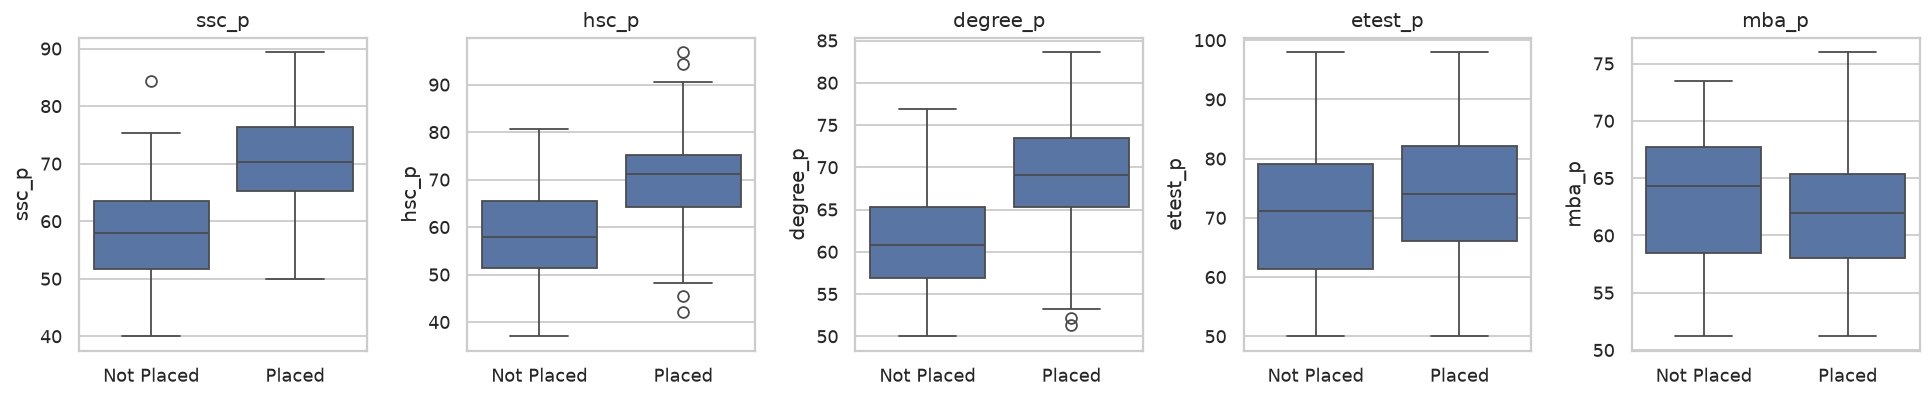
\includegraphics[width=\linewidth]{eda_lab/figs/pl_box_by_status.png}\end{center}
\begin{lstlisting}
for c in pct:
    a, b = pl.loc[pl.placed == 1, c], pl.loc[pl.placed == 0, c]
    t, p = stats.ttest_ind(a, b, equal_var=False)       # Welch's t-test
\end{lstlisting}
\outlabel
\begin{lstlisting}[style=out]
ssc_p     placed mean  71.2 vs  57.8  Welch t = 10.39, p = 8.3e-19
hsc_p     placed mean  69.9 vs  58.5  Welch t =  7.69, p = 3.8e-12
degree_p  placed mean  68.9 vs  61.5  Welch t =  7.54, p = 5.8e-12
etest_p   placed mean  73.8 vs  71.2  Welch t =  1.46, p = 0.15
mba_p     placed mean  61.9 vs  63.1  Welch t = -1.61, p = 0.11
\end{lstlisting}
\textbf{Reading}: the box plots barely overlap for 10th, 12th and degree percentages; placed students score about 13 points higher in school. The employability test and MBA
percentage do not differ significantly. \textbf{Interview insight}: recruiters appear to screen on the long-run academic record; the MBA score itself is not what separates the
groups. (Ask: is that because MBA grading is compressed? Its sd is only 5.4.)

\section{Step 7: thresholds a placement cell can act on}
\begin{lstlisting}
rate_by(pl, "ssc_p", "placed", bins=[0, 55, 60, 65, 70, 75, 100])
\end{lstlisting}
\outlabel
\begin{lstlisting}[style=out]
            rate   n
(0, 55]    0.161  31
(55, 60]   0.346  26
(60, 65]   0.625  32
(65, 70]   0.864  44
(70, 75]   0.806  31
(75, 100]  0.961  51
\end{lstlisting}
\begin{center}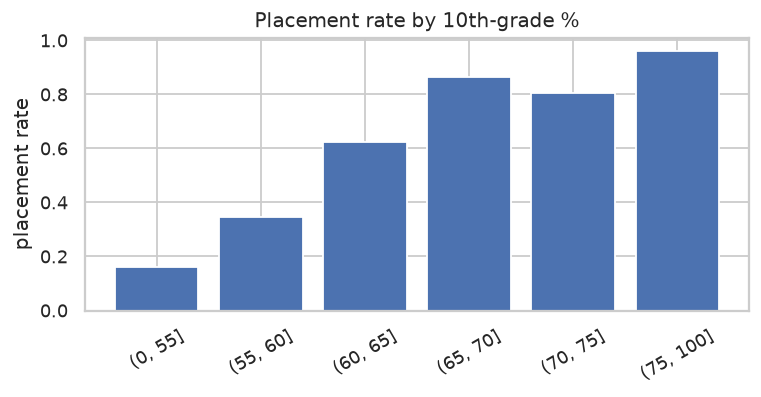
\includegraphics[width=0.55\linewidth]{eda_lab/figs/pl_rate_ssc.png}\end{center}
\textbf{Reading}: placement climbs steeply from 16\% (10th-grade score $\le$55) to 96\% (above 75), with the biggest jump around 60--65. Below 60, about two-thirds are not
placed: a clear, explainable at-risk segment for coaching. The small dip at 70--75 (31 students) is within noise. The curve is S-shaped, which is exactly what logistic
regression models.

\section{Step 8: categorical features}
\begin{lstlisting}
cats = ["gender", "ssc_b", "hsc_b", "hsc_s", "degree_t", "workex", "specialisation"]
for c in cats:
    t = pd.crosstab(pl[c], pl["placed"]); chi2, p, *_ = stats.chi2_contingency(t)
    print(c, round(cramers_v(pl[c], pl["placed"]), 3), round(p, 4), rate_by(pl, c, "placed")["rate"].to_dict())
\end{lstlisting}
\outlabel
\begin{lstlisting}[style=out]
feature         cramers_v  chi2_p  placement rate by level
workex              0.171   0.019  No 0.627 | Yes 0.800
specialisation      0.164   0.024  Mkt&Fin 0.750 | Mkt&HR 0.596
hsc_s               0.060   0.678  Arts 0.800 (n=10) | Commerce 0.681 | Science 0.663
degree_t            0.048   0.784  Comm&Mgmt 0.696 | Others 0.647 (n=17) | Sci&Tech 0.650
gender              0.027   0.810  F 0.662 | M 0.688
ssc_b               0.027   0.798  Central 0.667 | Others 0.692
hsc_b               0.000   1.000  Central 0.679 | Others 0.679
\end{lstlisting}
\begin{center}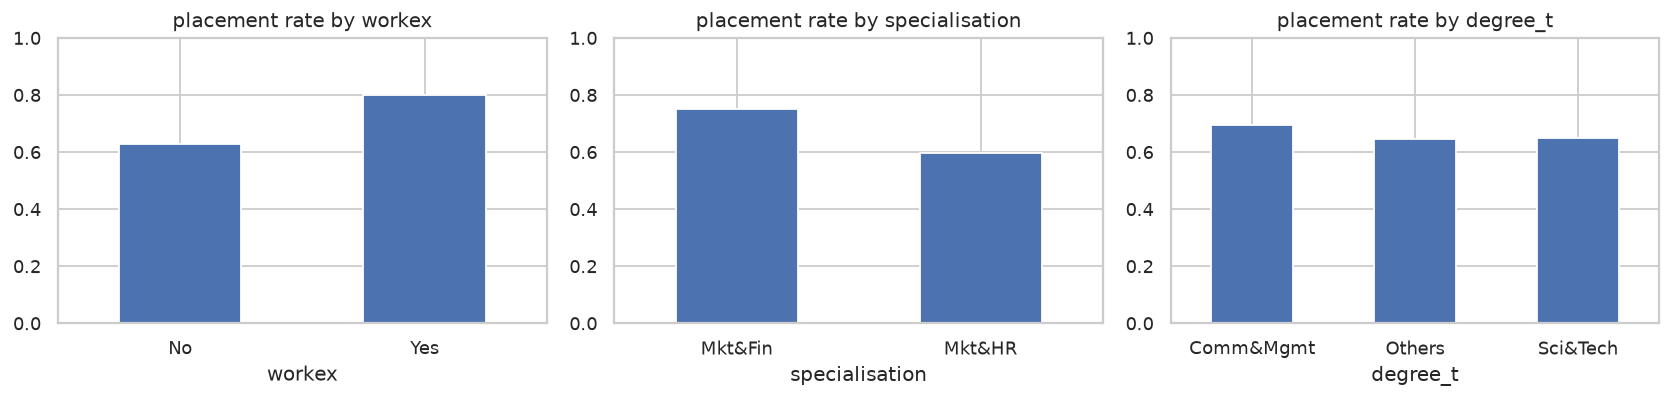
\includegraphics[width=\linewidth]{eda_lab/figs/pl_cat_rates.png}\end{center}
\begin{lstlisting}
pd.crosstab(pl["workex"], pl["specialisation"], values=pl["placed"], aggfunc="mean").round(2)
\end{lstlisting}
\outlabel
\begin{lstlisting}[style=out]
specialisation  Mkt&Fin  Mkt&HR
workex
No                 0.70    0.55
Yes                0.85    0.73
\end{lstlisting}
\textbf{Reading}: work experience (+17 points) and Mkt\&Fin specialisation (+15 points) are the only categorical features with a significant association. The effects
add up: Mkt\&HR students without work experience are placed at 55\%, Mkt\&Fin with experience at 85\%. Boards, stream and degree type show no meaningful difference.
\code{hsc\_s = Arts} (80\%) rests on only 10 students: do not read anything into it.

\section{Step 9: correlations and multicollinearity}
\begin{lstlisting}
sns.heatmap(pl[pct + ["placed"]].corr(), annot=True, fmt=".2f", cmap="coolwarm", vmin=-1, vmax=1)
vif(pl[pct])
\end{lstlisting}
\begin{center}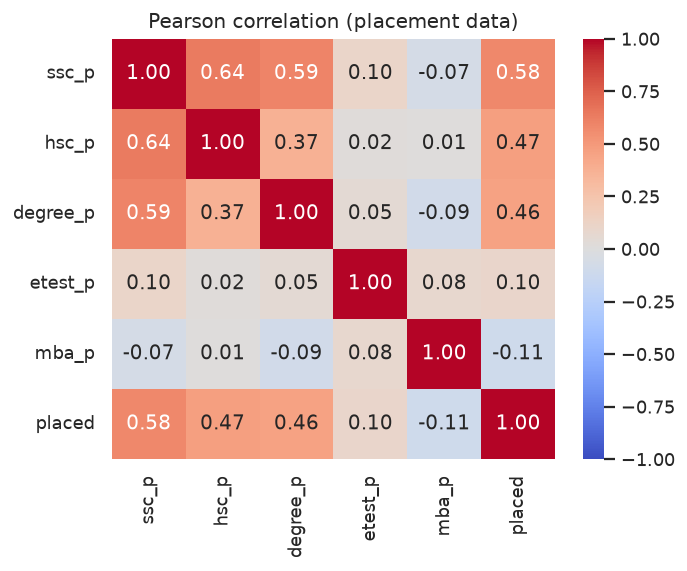
\includegraphics[width=0.55\linewidth]{eda_lab/figs/pl_corr.png}\end{center}
\outlabel
\begin{lstlisting}[style=out]
ssc_p 2.28   hsc_p 1.70   degree_p 1.55   etest_p 1.02   mba_p 1.02
\end{lstlisting}
\textbf{Reading}: the three academic scores correlate with each other (0.37--0.64: a shared ``academic ability'' factor) and with placement; employability test and MBA
percentage are unrelated to everything. All VIFs are below 2.3, so multicollinearity is not a problem for a logistic regression; coefficients will be stable.

\section{Step 10: multivariate view and a sanity-check model}
\begin{lstlisting}
sns.scatterplot(data=pl, x="ssc_p", y="degree_p", hue="status", style="workex")
X = pd.get_dummies(pl[pct + ["workex", "specialisation", "gender"]], drop_first=True).astype(float)
auc = cross_val_score(make_pipeline(StandardScaler(), LogisticRegression(max_iter=1000)),
                      X, pl["placed"], cv=StratifiedKFold(5, shuffle=True, random_state=0), scoring="roc_auc")
\end{lstlisting}
\begin{center}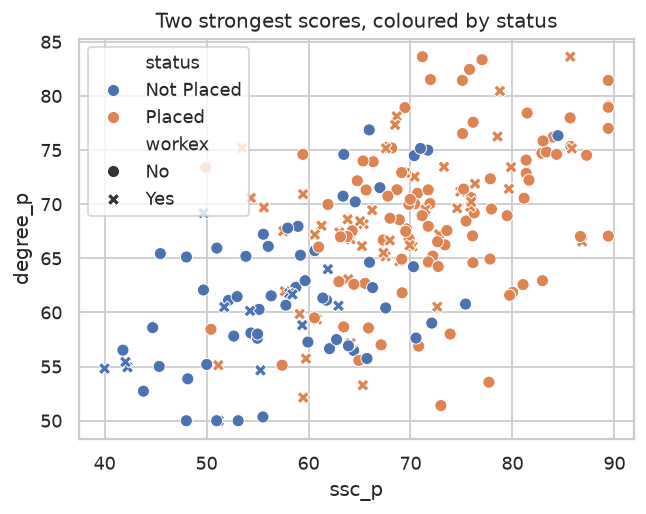
\includegraphics[width=0.55\linewidth]{eda_lab/figs/pl_scatter.png}\end{center}
\outlabel
\begin{lstlisting}[style=out]
CV ROC AUC using EDA-selected features (no salary): 0.916 +/- 0.024
\end{lstlisting}
\textbf{Reading}: placed students cluster in the upper-right of the school-vs-degree plane, with a fuzzy diagonal boundary: a linear model fits. Without salary, a 5-fold
cross-validated logistic regression reaches AUC 0.92, honestly; with salary it would reach 1.0, dishonestly.

\section{Step 11: the summary you say at the end}
\begin{enumerate}
\item 215 students, no duplicates, all percentages valid, so no outlier removal.
\item \textbf{Salary is recorded only for placed students: a perfect but leaky predictor. Drop it for placement; use it only for a separate salary model on placed students.}
\item 68\% placed: mildly imbalanced; report precision/recall/F1 and AUC, stratify splits.
\item 10th-grade, 12th-grade and degree percentages are the strongest drivers (point-biserial 0.46--0.58); employability test and MBA percentage add little.
\item Work experience and Mkt\&Fin specialisation raise placement by about 15 points each, additively; boards and stream do not matter.
\item Placement rises steeply with 10th-grade score: students below 60 form a clear at-risk group.
\item No multicollinearity concerns; a logistic regression on these features gives CV AUC $\approx$0.92.
\item Salary (for the separate question) is right-skewed: log-transform; higher with work experience; a gender gap worth investigating with controls.
\end{enumerate}

\stuck{Kaggle: Campus Recruitment dataset (search)}{\yts{campus+recruitment+placement+data+analysis+python+EDA}}
\section{Interview questions}

\begin{qa}{\pyq{Round 3, reported} In the placement data, if the package (salary) is given, can you tell whether the student was placed? What do you do with the column?}
\oneline{Yes, perfectly: salary is filled only for placed students, so ``salary present'' predicts placement with 100\% accuracy; because it is recorded after the outcome and is
unavailable at prediction time, it is target leakage and must be dropped from the placement model.}
\why Show it with two lines: the fraction of missing salary by status (1.0 vs 0.0) and the crosstab of \code{salary.notna()} vs status (no off-diagonal cells). Then explain timing:
the model is meant to be used before placement. Mention the legitimate use: a separate salary regression on placed students, or a two-part expected-salary model.
\pushes \emph{``What if salary were only partly missing for placed students?''} Then it is still leaky (its presence is mostly determined by the outcome) and also messy; the answer does not
change. \emph{``How would a model reveal the leak if you missed it?''} Near-perfect AUC and a dominant importance for salary or its missing indicator.
\end{qa}

\begin{qa}{Would you impute the missing salaries? Why or why not?}
\oneline{No: for non-placed students salary is not unknown, it is not applicable; there is nothing to estimate, and any imputed value or indicator would still encode the outcome.}
\end{qa}

\begin{qa}{Which scores matter for placement, and how did you establish it?}
\oneline{10th, 12th and degree percentages (point-biserial 0.58, 0.48, 0.46; Welch t-tests with $p<10^{-11}$; non-overlapping box plots), while employability test and MBA percentage show
no significant difference.}
\end{qa}

\begin{qa}{\deep MBA percentage does not differ between placed and non-placed students. Does that mean the MBA does not matter?}
\oneline{No: it means variation \emph{in MBA percentage among MBA students} does not separate outcomes in this sample, perhaps because MBA grades are compressed (sd 5.4) or recruiters screen
on earlier records; everyone in the data has the MBA, so its overall value cannot be measured here.}
\end{qa}

\begin{qa}{How would you present the 10th-grade threshold finding to a placement cell?}
\oneline{As a simple, explainable at-risk rule with uncertainty: ``students with 10th-grade scores below 60 are placed only 16--35\% of the time (57 students), versus over 80\% above 65;
prioritise them for coaching and mock interviews'', and propose measuring whether coaching changes their rate.}
\end{qa}

\begin{qa}{\deep The \code{hsc\_s = Arts} group has an 80\% placement rate, the highest. Would you add ``Arts stream'' as an important finding?}
\oneline{No: it is based on 10 students, and the chi-square test for stream is far from significant ($p = 0.68$); a difference of one or two students would change it; report it with its
count and treat it as noise.}
\end{qa}

\begin{qa}{How would you check whether the gender gap in salary is real?}
\oneline{Compare medians with confidence intervals (bootstrap), then control for specialisation, work experience and scores with a regression of log salary, check sample sizes, and say
clearly that an observational difference is not proof of discrimination or of its absence.}
\end{qa}

\begin{qa}{After this EDA, what model and preprocessing would you choose?}
\oneline{Drop \code{sl\_no} and \code{salary}; one-hot encode the categoricals (drop one level for an unregularised model); standardise the scores; stratified split; logistic regression as
the interpretable baseline (CV AUC $\approx$0.92), compared with a small random forest; report the confusion matrix, precision, recall, F1 and AUC.}
\end{qa}
